\documentclass[11pt,a4paper]{article}

\usepackage[margin=1in]{geometry}
\usepackage{amsmath, amssymb, mathtools}
\usepackage{fontspec}
\IfFontExistsTF{Times New Roman}
  {\setmainfont{Times New Roman}}
  {\setmainfont{Liberation Serif}}
\IfFontExistsTF{Arial}
  {\setsansfont{Arial}}
  {\setsansfont{Liberation Sans}}
\usepackage{newunicodechar}
\newunicodechar{≈}{\ensuremath{\approx}}
\newunicodechar{≤}{\ensuremath{\leq}}
\newunicodechar{≥}{\ensuremath{\geq}}
\newunicodechar{×}{\ensuremath{\times}}
\newunicodechar{−}{\ensuremath{-}}

\usepackage{xcolor}
\definecolor{headingcolor}{HTML}{1F4E79}
\definecolor{lightgray}{HTML}{666666}

\usepackage{setspace}
\onehalfspacing
\setlength{\parindent}{0pt}
\setlength{\parskip}{0.6em}

\usepackage{titlesec}
\titleformat{\section}
{\color{headingcolor}\sffamily\Large\bfseries}
{\thesection}{1em}{}
\titleformat{\subsection}
{\sffamily\large\bfseries}
{\thesubsection}{1em}{}

\usepackage{listings}
\lstset{
    basicstyle=\ttfamily\footnotesize,
    breaklines=true,
    columns=fullflexible,
    frame=single,
    framerule=0.4pt,
    showstringspaces=false,
    xleftmargin=0.4em,
    xrightmargin=0.4em,
    aboveskip=0.5em,
    belowskip=0.5em,
}

\usepackage{booktabs}
\usepackage{graphicx}
\usepackage{caption}
\captionsetup{font=small, labelfont=bf}

\newcommand{\courseheader}{
    \begin{center}
        {\sffamily\Large\bfseries CESE5040}\\[0.3em]
        {\sffamily High-Performance and AI Architectures}\\
        {\color{lightgray}2026 Q4}
    \end{center}
}

\newcommand{\Q}[1]{\subsection*{Question #1}}
\newcommand{\Qpart}[1]{\textbf{#1.}}

\begin{document}

\courseheader
\vspace{1em}

{\color{headingcolor}\sffamily\large\bfseries Student Information}

\textbf{Name:} Daniel Tyukov\\
\textbf{Student Number:} 5714699\\
\textbf{Lab:} Lab Assignment 6: The Inferior-Olive challenge

{\color{headingcolor}\sffamily\large\bfseries Notes}

\begin{itemize}\setlength\itemsep{0.1em}
    \item Model: de Gruijl extended-Hodgkin--Huxley IO cell, three compartments (soma, axon, dendrite) with all-to-all gap junctions; forward-Euler, $\delta = 10$\,\textmu s, $N$ cells.
    \item Hardware: laptop Intel Core Ultra 9 185H (22 threads) for the CPU backends; AWS Tesla T4 (16\,GB, 70\,W) for the GPU backend.
    \item Metric: mean wall-time \emph{per simulation step}, the quantity the brief's real-time budget constrains (one step per $\delta=10$\,\textmu s of brain time). The wall time to simulate 1\,s of brain time is this $\times\,10^5$ steps. Each point is the best of three warm runs; JIT compilation is excluded.
\end{itemize}

\vspace{0.5em}

\section*{\color{headingcolor}Lab Exercise 6}

% =========================================================================
\Q{6.1: Parameter exploration}

Each parameter was varied on its own (pairwise, against the defaults) and the morphology of the soma trace was measured. Table~\ref{tab:explore} summarises the effect; Figure~\ref{fig:morph} shows the two that change the dynamics qualitatively. Sub-threshold oscillations (STOs) remain near 6\,Hz throughout.

\begin{table}[h]
\centering
\small
\begin{tabular}{p{3.0cm}p{11.2cm}}
\toprule
Parameter (range) & Morphological effect \\
\midrule
\texttt{sim\_seconds} [0.5--2.0] & No change in shape: same $\sim$6\,Hz STO, $\sim$22\,mV peak-to-peak. Only the recorded window lengthens, and runtime grows in proportion to the step count. \\
\texttt{delta} [0.01--0.05] & Single-cell trace essentially unchanged (peak-to-peak 21.6$\to$21.7\,mV). A coarser step means fewer steps (faster) at a small accuracy cost; its stability cost only surfaces at large $N$ (Q6.2). \\
\texttt{n\_cells} [1--30], GJ on & The isolated cell swings $\pm$31\,mV; as the population grows the cells synchronise and each one's amplitude reduces to $\sim$22\,mV. Mean pairwise correlation rises $0.81\,(N{=}2)\to0.97\,(N{\geq}10)$. \\
\texttt{enable\_gapjunctions} ($N{=}30$) & Controls synchrony: on $\Rightarrow$ correlation $0.97$ and one shared rhythm; off $\Rightarrow$ correlation $0.26$, with cells on independent phases and larger individual swings (Fig.~\ref{fig:morph}b). \\
\texttt{g\_CaL} [0.7--2.0], $N{=}1$ & Sets the firing mode. At $0.7$ the cell only oscillates sub-threshold ($V_{\max}=-46$\,mV, no spikes); at $\geq1.8$ it fires full Ca-spikes ($V_{\max}=+41$\,mV, 7\,Hz, 112\,mV peak-to-peak), Fig.~\ref{fig:morph}a. \\
\texttt{I\_pulse10ms} [2--10], $N{=}30$ & Stimulus amplitude. At 2--5 it produces a sub-threshold deflection (peak-to-peak $22\to26$\,mV); at 8 it evokes a single spike; at 10 it drives an 8-spike burst and re-entrains the rhythm to $\sim$2\,Hz. \\
\bottomrule
\end{tabular}
\caption{Effect of each parameter on the simulator output. STO frequency stays near 6\,Hz; the parameters that reshape the trace are \texttt{g\_CaL} (firing mode), the gap junctions (synchrony) and a strong \texttt{I\_pulse10ms} (evoked spikes).}
\label{tab:explore}
\end{table}

\begin{figure}[h]
\centering
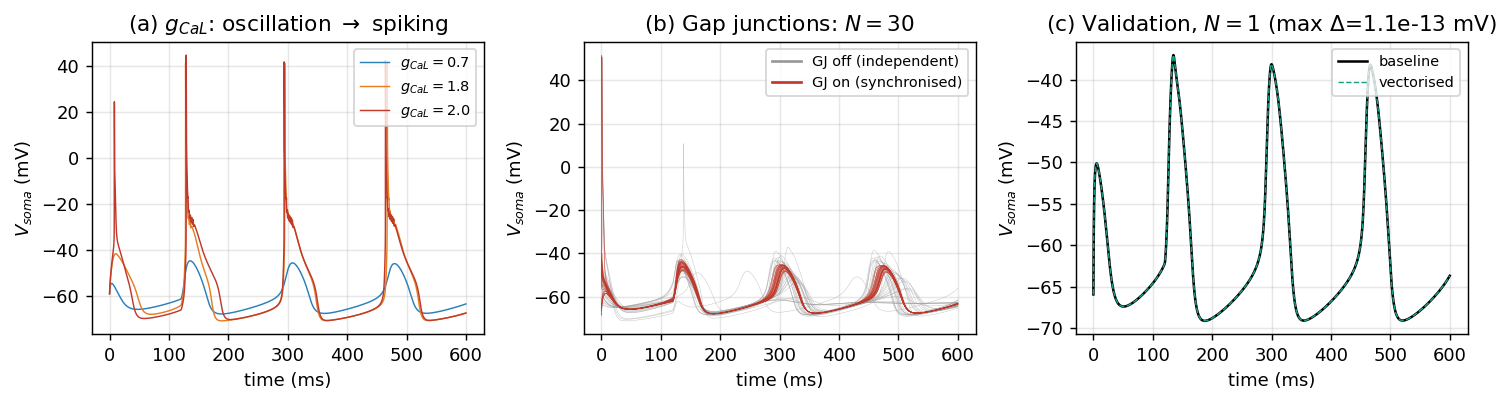
\includegraphics[width=\linewidth]{../figures/fig_morphology.png}
\caption{(a) \texttt{g\_CaL} switches the cell from a sub-threshold oscillator (blue) to a Ca-spiking cell (orange/red). (b) Gap junctions bring 30 randomly-initialised cells (grey, independent) into one synchronised rhythm (red). (c) Validation: the vectorised backend reproduces the baseline trace to $1.1\times10^{-13}$\,mV at $N=1$.}
\label{fig:morph}
\end{figure}

% =========================================================================
\Q{6.2: Accelerating the simulator}

\Qpart{1 (Pen-and-paper analysis and profiling)}
Per time step the solver touches each of the $N$ cells once and, for each cell, updates three compartments. A compartment update is a fixed block of $\sim$40 \texttt{exp()} evaluations and arithmetic, i.e.\ $O(1)$ work, so the channel and compartment cost is $O(N)$ per step. The gap junction is the exception. As written it is a double loop: cell $i$ sums $C_{\text{gap}}(V_d^i - V_d^j)$ over every other cell, which is $O(N)$ per cell and therefore
\[
\text{cost per step} \;=\; \underbrace{O(N)}_{\text{compartments}} \;+\; \underbrace{O(N^2)}_{\text{gap junctions}}, \qquad
\text{total} \;=\; O\!\big(T\,N^2\big),\quad T=\tfrac{1000\,\texttt{sim\_seconds}}{\delta}.
\]
With the default $T=10^5$ steps the quadratic term overtakes the linear one beyond a few tens of cells. Profiling the sequential code (cProfile, $N=30$) agrees: \texttt{update\_dend}, the function holding the gap-junction loop, takes 49\,\% of the time, \texttt{update\_soma} 34\,\%, \texttt{update\_axon} 16\,\% (Fig.~\ref{fig:prof}a), and the measured per-step time bends away from $O(N)$ toward $O(N^2)$ as $N$ grows (Fig.~\ref{fig:prof}b). The 1.8\,M Python function calls per 5000 steps are the constant-factor overhead on top.

\textbf{The key observation} is that the all-to-all sum collapses. For uniform linear coupling,
\[
\sum_{j\neq i} C_{\text{gap}}\big(V_d^i - V_d^j\big) \;=\; C_{\text{gap}}\Big(N\,V_d^i - \textstyle\sum_{j} V_d^j\Big),
\]
so one global sum $\Sigma=\sum_j V_d^j$, formed once per step in $O(N)$, serves every cell in $O(1)$. The gap junction drops from $O(N^2)$ to $O(N)$ \emph{exactly}. This is the ``partition in space'' point from the lectures: the coupling links all cells every step, but its structure is a mean field.

\begin{figure}[h]
\centering
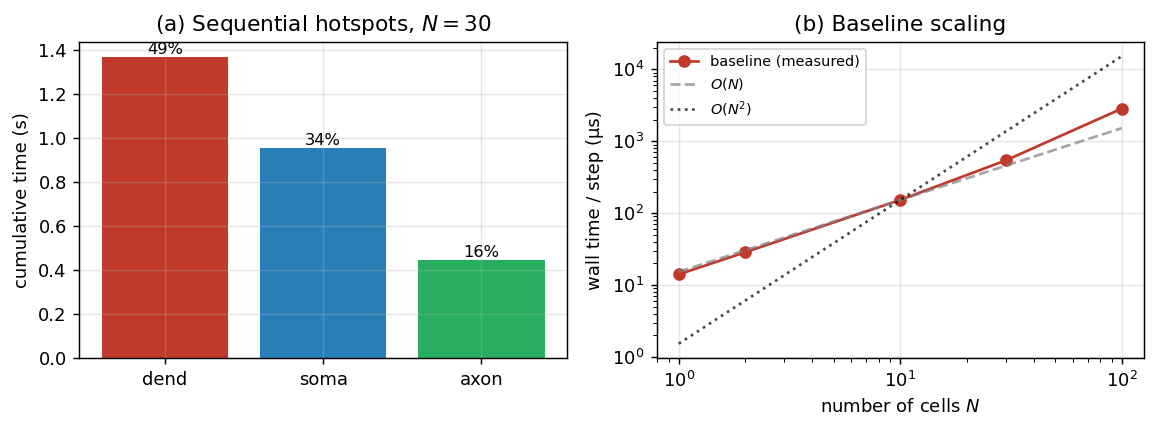
\includegraphics[width=\linewidth]{../figures/fig_profile.png}
\caption{(a) Sequential hotspots at $N=30$: the dendrite update (gap junctions) dominates. (b) Baseline per-step time, measured against $O(N)$ and $O(N^2)$ guides anchored at $N=10$; the curve leaves the linear guide as the quadratic gap-junction term takes over.}
\label{fig:prof}
\end{figure}

\Qpart{2 (Plan of attack)}
The techniques are the ones built up over Labs 2--5. Multiprocessing (Lab 2) is left out on purpose: Lab 2 showed that for fine-grained per-timestep work the process pool's IPC and serialisation cost exceeds the few microseconds of real work per step, so it loses to a vectorised kernel. The right family for this workload is therefore vectorise $\to$ JIT $\to$ GPU.
\begin{enumerate}\setlength\itemsep{0.1em}
    \item \textbf{Take the interpreter out of the hot loop.} Vectorise across cells, as in Lab 3's \texttt{tvb\_vec}: hold each state variable as a length-$N$ array and make one timestep $\sim$30 array operations instead of $3N$ Python calls (NumPy).
    \item \textbf{Kill the $O(N^2)$.} Replace the gap-junction loop with the $O(N)$ mean-field sum above. Lab 3 made the same point in reverse: porting before refactoring the per-centre loop just launches more tiny kernels.
    \item \textbf{Compile the step.} Numba \texttt{@njit} (\texttt{fastmath}) for low-overhead single-core machine code; JAX/XLA \texttt{jit}+\texttt{lax.scan} for a fused kernel that also runs on the GPU unchanged (both used in Labs 3--5).
    \item \textbf{Offload the tail to the T4.} Run the same JAX program on the GPU for large $N$, the GPU path from Lab 3 (CuPy) and Lab 5 (JAX on the T4).
    \item \textbf{Stay faithful.} Keep forward-Euler and the intra-cell update order identical to the baseline so the result can be validated (matches to round-off at $N=1$, Fig.~\ref{fig:morph}c; the only change at $N>1$ is the gap junction moving from a within-step Gauss--Seidel sweep to a Jacobi update, which leaves the dynamics indistinguishable: max $\Delta=0.02$\,mV, correlation $1.0000$ at $N=30$).
\end{enumerate}

\Qpart{3 (Accelerated results)}
All four accelerated backends run the full sweep, including the $10^5$-cell case the sequential code cannot reach. Table~\ref{tab:sweep} and Figure~\ref{fig:scaling} give the per-step cost.

\begin{table}[h]
\centering
\small
\begin{tabular}{lrrrrrrrr}
\toprule
$N$ & 1 & 2 & 10 & 30 & 100 & 1000 & 10000 & 100000 \\
\midrule
Baseline        & 14.1 & 28.7 & 152.7 & 543.8 & 2852.7 & n/a & n/a & n/a \\
NumPy (vec.)    & 76.3 & 76.4 & 80.9 & 85.0 & 93.2 & 243.9 & 1369 & 15056 \\
Numba (CPU)     & \textbf{0.09} & \textbf{0.19} & \textbf{0.93} & \textbf{2.73} & \textbf{9.04} & 90.7 & 1111 & 11183 \\
JAX/XLA (CPU)   & 10.6 & 11.9 & 14.3 & 14.6 & 16.4 & \textbf{32.2} & 160.2 & 600.7 \\
JAX/XLA (T4 GPU)& 60.9 & 46.0 & 45.7 & 47.2 & 46.1 & 46.9 & \textbf{46.9} & \textbf{112.5} \\
\bottomrule
\end{tabular}
\caption{Wall time per step (\textmu s) versus population size. Bold marks the fastest backend at each $N$. The 1-second-brain-time wall is these values $\times\,0.1$\,s (e.g.\ baseline $N=30$: 54.4\,s; Numba: 0.27\,s; GPU $N=10^5$: 11.3\,s).}
\label{tab:sweep}
\end{table}

\begin{figure}[h]
\centering
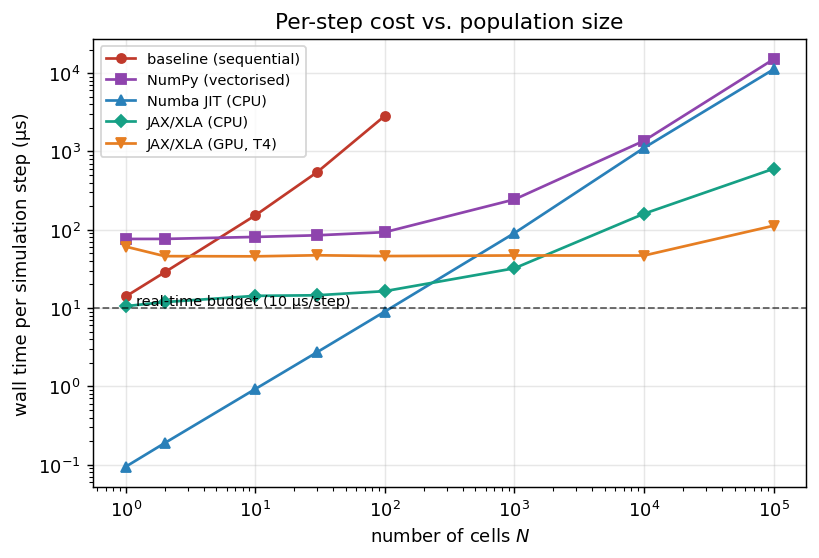
\includegraphics[width=0.74\linewidth]{../figures/fig_scaling.png}
\caption{Per-step cost versus $N$ (log-log). Numba is the only backend under the 10\,\textmu s real-time budget (dashed), and wins up to a few hundred cells; JAX/XLA on CPU then overtakes it; the T4 stays flat at $\sim$46\,\textmu s out to $N=10^4$ and wins the large-$N$ tail.}
\label{fig:scaling}
\end{figure}

\Qpart{4 (Analysis: were the findings what I expected?)}
Mostly as expected; the exception is the stability limit noted below.

\emph{Speedups.} Removing the interpreter and the $O(N^2)$ term gives large gains. At $N=30$, Numba is 199$\times$ the baseline, JAX/XLA-CPU 37$\times$, plain vectorised NumPy 6.4$\times$; at $N=100$ Numba reaches 316$\times$. At $N=10^5$, which the baseline cannot reach in reasonable time, the T4 is 99$\times$ faster than Numba and 134$\times$ faster than NumPy.

\emph{Three regimes, set by the latency--throughput trade-off from the lectures.}
\begin{itemize}\setlength\itemsep{0.1em}
    \item \textbf{Small $N$ ($\lesssim10^2$): Numba wins.} With no dispatch overhead it runs at 0.09--9\,\textmu s/step and is the \emph{only} backend inside the 10\,\textmu s real-time budget, so a single core can simulate up to $\sim$100 IO cells in real time.
    \item \textbf{Mid $N$ ($\sim10^3$): JAX/XLA-CPU wins.} Once the arrays are large enough to amortise its $\sim$10\,\textmu s call overhead, XLA's fused, SIMD-vectorised kernel beats Numba's scalar loop.
    \item \textbf{Large $N$ ($\gtrsim3\times10^3$): the GPU wins.} The T4's per-step time is \emph{flat} at $\sim$46\,\textmu s all the way to $N=10^4$: the work is too small to fill 2560 CUDA cores, so the step is bound by kernel-launch latency, not arithmetic. Only at $N=10^5$ does compute finally show. This repeats Lab 3's CuPy result, where each T4 launch cost $\sim$6--10\,\textmu s and the GPU only paid off at TVB998; here the same crossover lands near $N=3000$. The GPU never beats the 10\,\textmu s latency, but its throughput dominates everything else offline.
\end{itemize}
This is consistent with the lecture framing that brain simulation is \emph{not} embarrassingly parallel: the per-step global sum $\Sigma$ is a synchronisation barrier across all cells, so the parallelism is in space (cells), never in time (steps stay sequential).

\emph{Stability, not compute, becomes the binding limit.} The mean-field reduction makes even $10^5$ cells cheap to compute, so the limiting factor at large $N$ is numerical. With a fixed $C_{\text{gap}}$ the coupling current grows as $C_{\text{gap}}\,N\,(V_d^i-\overline{V_d})$, and forward-Euler stability requires $\delta\,C_{\text{gap}}\,N < 2$, i.e.\ $N < 2/(\delta\,C_{\text{gap}}) = 4000$. This matches the measurement: the trajectory is stable to $N=3000$ and diverges at $N=4000$. Beyond that the per-step timings remain valid (the arithmetic is identical) but the dynamics are non-physical unless the coupling is normalised ($C_{\text{gap}}/N$) or $\delta$ is reduced. The acceleration therefore reaches a modelling limit that the sequential code was too slow to encounter.

% =========================================================================
\vspace{1em}

{\color{headingcolor}\sffamily\large\bfseries LLM Usage Disclosure}

\vspace{0.3em}

I used Claude Code on this lab for:
\begin{itemize}\setlength\itemsep{0.1em}
    \item Cross-checking the $O(N^2)\!\to\!O(N)$ gap-junction derivation and the forward-Euler stability bound.
    \item Researching the acceleration techniques against the lecture and prior-lab material, and editing the report for concision.
\end{itemize}

\end{document}
